\documentclass{CjC}
\usepackage{don}
\usepackage{tikz}
\usepackage{pgf-pie}
\usepackage{pgfplots}
\usepackage{subfig}

% ==================================================
\begin{document}

% 标题部分
\begin{center}
\zihao{2-}{\fangsong \textbf{对成渝双圈科技与社会协调发展的探讨}}

\vspace{10pt}

\zihao{4-}{\kaishu Koorye$^1$}

\vspace{10pt}

\zihao{5}{\songti (1. 电子科技大学,计算机科学与工程学院,成都\ 611731)}
\end{center}

\vspace{10pt}

% ==================================================
% 摘要部分
\songti

\textbf{摘要:} {\kaishu 《成渝地区双城经济圈建设规划纲要》是中共中央印发的重要文件,其目的是促进成渝地区发展特色双城经济圈,筑城全国高质量发展的新兴一极和动力来源。其中,科技与社会协调发展是成渝双圈国家纲要的重要组成部分,对于推动成渝双城经济圈建设具有重要意义。本文旨在探讨成渝双圈国家纲要中科技与社会协调发展的关系,分析科技与社会协调发展在成渝双圈国家纲要中的作用,探讨科技与社会的相互作用,分析成渝双圈国家纲要实施中的挑战与机遇,为推动成渝双城经济圈建设提供参考。}

\textbf{关键词:} 成渝双圈;国家纲要;科技创新;社会发展;协调发展

\textbf{中图分类号:} \textbf{NO31} \quad \textbf{文献识别码:} \textbf{A}

\vspace{10pt}

% ==================================================
% 正文部分
\section{引言}

% 介绍主题
《成渝地区双城经济圈建设规划纲要》是中共中央印发的重要文件,其目的是促进成渝地区发展特色双城经济圈,筑城全国高质量发展的新兴一极和动力来源。其中,科技与社会协调发展是成渝双圈国家纲要的重要组成部分,对于推动成渝双城经济圈建设具有重要意义。

% 背景信息
成都和重庆是我国西南地区的两大城市,也是西部地区的核心经济门户\cite{戴宾2005成渝经济区与成渝城市集群}。成都市坐落在中国西南地区四川盆地中部,是四川省的首府都市,也是中国西部地区重要的政治、经济、文化中心。重庆市位居中国中部长江上游,地处中国西南地区,作为直辖市具有省级地位。成渝双城经济圈是成都和重庆两大城市共同发展的重要载体,是推动成渝地区经济社会协调发展的重要平台。

% 本文目标
本文旨在探讨成渝双圈国家纲要中科技与社会协调发展的关系,分析科技与社会协调发展在成渝双圈国家纲要中的作用,探讨科技与社会的相互作用,分析成渝双圈国家纲要实施中的挑战与机遇,为推动成渝双城经济圈建设提供参考。

% 本文结构
本文共分为四个部分:第一部分为成渝双圈国家纲要的背景介绍,介绍成渝双圈国家纲要的重要性;第二部分为成渝双圈科技与社会协调发展的概述,分析科技与社会协调发展在成渝双圈国家纲要中的作用;第三部分为成渝双圈国家纲要实施中的挑战与解决方案;第四部分为结论,总结全文内容。

\section{纲要概述}

\begin{figure}[h]
\centering
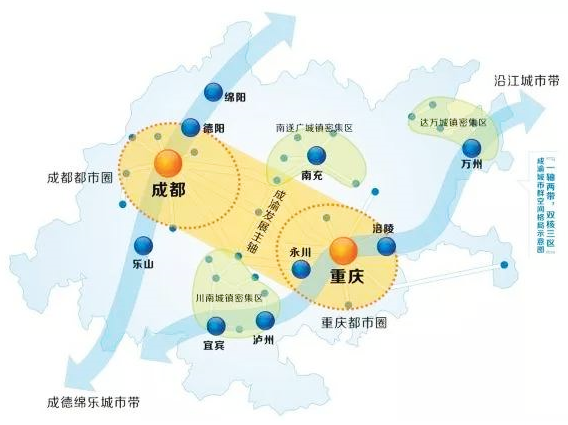
\includegraphics[width=0.7\textwidth]{pics/成渝双城经济圈.png}
\caption{成渝双城经济圈}
\label{fig:map}
\end{figure}

《成渝双圈双城经济圈建设规划纲要》(后面简称《纲要》)是2021年10月20日由中央印发的关于成渝区域建设的纲领性文件,如图\ref{fig:map}所示,该文件将重庆市中心城区及各区县,成都、自贡、泸州、德阳、绵阳等15个市,总面积18.5万平方千米,划定为双城经济圈。《纲要》提出到2025年,成渝区域将显著提升经济能力;到2035年,实现具备国际影响力的经济中心。《纲要》明确了建设双城经济圈的新发展模式,包括联合打造现代化基础设施网络、共同发展现代产业系统、建立全国范围内有影响力的科技创新中心,以及创建国际级的消费旅游目的地。此外,还强调了共同构建长江上游的生态防线,这些举措对促进成渝地区经济和社会的协调发展具有指导意义。

《纲要》在成渝地区的远景规划中扮演着至关重要的角色。这份规划明确了成渝地区双城经济圈的战略定位和发展目标,旨在打造一个具有全国影响力的重要经济中心、科技创新中心、改革开放新高地以及高品质生活宜居地。这一愿景将引领着成渝地区的未来发展,为我们的城市和人民创造更加美好的明天。《纲要》为成渝地区的未来发展绘制了蓝图,包括基础设施建设、产业体系协同、科技创新、生态环境保护等多个方面的详细规划。《纲要》推动了重庆和成都两个中心城市的协同发展,以及周边城市和乡村的均衡发展,促进了区域内资源的合理配置和高效利用。《纲要》加速了对外开放大通道的构建,提高了区域在国际分工体系中的竞争力,对于“一带一路”和长江经济带的协同发展具有积极意义。这一规划将有助于构建一个优势互补、高质量发展的区域经济格局,为成渝地区的繁荣与进步创造更加有利的条件。

在《纲要》中,科技与社会的协调发展被视为成渝双城经济圈的重要组成部分。科技创新作为推动经济社会发展的关键动力,对实现高质量发展至关重要。科技创新不仅能够提高生产效率,优化产业结构,增强企业竞争力,还能推动整体经济增长。因此,科技创新被视为成渝双城经济圈建设的核心内容,是实现经济社会协调发展的重要手段之一。而社会发展则扮演着科技创新的重要保障角色,同时也是科技创新的重要应用场景。社会发展有助于基础设施建设、产业体系协同发展以及生态环境保护等方面的协调发展,从而提升人民的幸福水平。科技与社会之间形成了相辅相成、相互促进的关系,共同推动了成渝双城经济圈的建设和繁荣。

\section{成渝双圈科技与社会的协调发展}

在成渝双城经济圈中,科技与社会协调发展是其中的重要组成部分。本章节将从科技与社会协调发展的概念、科技创新在成渝双圈国家纲要中的角色、社会发展在成渝双圈国家纲要中的重要性、科技与社会协调发展的互动关系等方面进行探讨。

\subsection{科技创新在成渝双圈国家纲要中的角色}

\begin{figure}[h]
\subfloat[我国各地区科研经费占比]{
    \centering
    \begin{tikzpicture}
    \pie[sum=auto, explode = 0.1, radius=2, color={blue!50, green!50, red!50, yellow!50}]{68/东部地区, 15/中部地区, 13/西部地区, 4/东北地区}
    \end{tikzpicture}
}
\subfloat[我国各主要城市科研经费]{
    \centering
    \begin{tikzpicture}
    \begin{axis}[
        ybar,
        bar width=0.3cm,
        width=0.5\textwidth,
        height=0.4\textwidth,
        ymin=0,
        ymax=450,
        ylabel={科研经费(亿元)},
        symbolic x coords={深圳, 上海, 北京, 天津, 广州, 合肥, 苏州, 武汉, 杭州, 宁波, 南京, 芜湖, 重庆, 成都, 无锡},
        xtick=data,
        nodes near coords,
        nodes near coords align={vertical},
        x tick label style={rotate=45, anchor=east},
        enlarge x limits=0.05,
        enlarge y limits=0.0,
        legend style={at={(0.5,-0.2)}, anchor=north, legend columns=-1},
    ]
    \addplot coordinates {(深圳, 404) (上海, 342) (北京, 286) (天津, 125) (广州, 113) (合肥, 102) (苏州, 95) (武汉, 86) (杭州, 75) (宁波, 57) (南京, 53) (芜湖, 52) (重庆, 52) (成都, 46) (无锡, 37)};
    \end{axis}
    \end{tikzpicture}
}
\caption{我国各地区和主要城市科研经费概况}
\label{fig:research}
\end{figure}

科技创新,既包括科学研究,也涵盖了技术创新。前者是一项原创性的科学探索,涉及新观点的提出和新技术领域的开拓;而后者则是将科学知识转化为实际应用,推动科技进步,提升社会生产力水平。当前,我国正处于经济高速发展向高质量发展的关键转型时期,科技创新成为实现这一目标的关键手段。科技创新不仅能够提高生产效率,优化产业结构,增强企业竞争力,还能推动整体经济增长。因此,科技创新被视为成渝双城经济圈建设的核心内容之一。

目前,我国西部城市面临科技水平相对落后、创新能力不足的问题\cite{游光荣2001我国地区科技竞争力研究,郭新艳2004基于}。如图\ref{fig:research}所示,我国各地区科研经费占比不均衡,东部地区科研经费占比较高,而西部地区科研经费占比较低。我国各主要城市科研经费也存在差异,深圳、上海、北京等东部城市科研经费较高,而重庆、成都等西部城市仅占很小的一部分。这说明我国西部城市科技创新水平相对较低,需要加大科研经费投入,提高科技创新能力。此外,我国西部城市科技创新人才相对匮乏,科技领军人才不足,院士数量仅为东部城市的1/5;“双一流”大学、国家重点实验室等机构数量相对不足,仅为京津冀和长三角地区的1/4\cite{冯静颖2006西部科技人才开发的问题与对策}。这些现象说明我国西部城市在科技创新方面存在较大的差距,需要加大科技创新力度,提高科技创新水平。

根据《纲要》要求,成渝双圈将实现以下几个科技创新目标:打造开放创新实验区,建设国家级科技创新中心,推动科技成果转化;深度融入长江经济带发展大战略,与东部城市开展科技创新合作,加强科技创新人才培养;打造综合性科学中心,建设世界级重大科技基础设施群和世界一流高校科研机构聚集区,推动科技创新成果转化。为了实现上述目标,中央将给予成渝双城经济圈更多的政策支持,包括赋予更大创新自主权、支持重大科技项目建设、推动成渝两地科创协同发展等。这些政策措施将有助于提高成渝双城经济圈的科技创新能力,建成具有国际影响力的科技创新中心。

成都和重庆,作为中国西部地区的两个重要城市,近年来在科技创新领域取得了显著进展。成都孕育了众多国家级的科技创新示范区,如四川天府国际生物城、未来科技城和成都高新技术产业开发区。与此同时,重庆两江新区、重庆高新技术产业开发区和重庆大学城等示范区的建立,标志着这座城市在科技创新的道路上迈出了坚实的步伐。这些示范区不仅推动了科技创新的发展,还促进了科技成果的应用和转化,未来,成渝地区将持续深化科技创新合作,加快科技成果的产业化进程,不断提升科技创新能力,为地区的经济和社会发展提供强有力的支撑,共同构建一个充满活力的双城经济圈。

\subsection{社会发展在成渝双圈国家纲要中的重要性}

\begin{figure}[h]
\subfloat[我国各地区GDP(亿元)及占比]{
    \centering
    \resizebox{0.5\textwidth}{!}{
    \begin{tikzpicture}
    \pie[sum=auto, explode = 0.1, radius=2, color={blue!50, green!50, red!50, yellow!50}]{52/东部地区:525733, 25/中部地区:261760, 17/西部地区:173753, 5/东北地区:51124}
    \end{tikzpicture}
    }
}
\subfloat[我国各主要省份GDP]{
    \centering
    \begin{tikzpicture}
    \begin{axis}[
        ybar,
        bar width=0.3cm,
        width=0.5\textwidth,
        height=0.3\textwidth,
        ymin=0,
        ymax=130000,
        ylabel={GDP(亿元)},
        symbolic x coords={广东, 江苏, 山东, 浙江, 河南, 四川},
        xtick=data,
        nodes near coords,
        nodes near coords align={vertical},
        x tick label style={rotate=45, anchor=east},
        enlarge x limits=0.2,
        enlarge y limits=0.0,
        legend style={at={(0.5,-0.2)}, anchor=north, legend columns=-1},
    ]
    \addplot coordinates {(广东, 110760) (江苏, 102700) (山东, 73129) (浙江, 64613) (河南, 54997) (四川, 48598)};
    \end{axis}
    \end{tikzpicture}
}
\\
\subfloat[我国各主要省级行政区城镇化率]{
    \centering
    \begin{tikzpicture}
    \begin{axis}[
        ybar,
        bar width=0.3cm,
        width=0.99\textwidth,
        height=0.3\textwidth,
        ymin=0,
        ymax=103,
        ylabel={城镇化率(\%)},
        symbolic x coords={全国, 上海, 北京, 天津, 广东, 江苏, 浙江, 辽宁, 重庆, 福建, 内蒙古, 宁夏, 黑龙江, 湖北, 山东, 陕西, 山西, 吉林, 江西, 河北, 海南, 青海, 湖南, 安徽, 四川, 新疆, 河南, 广西, 贵州, 甘肃, 云南, 西藏},
        xtick=data,
        nodes near coords,
        nodes near coords align={vertical},
        x tick label style={rotate=45, anchor=east},
        enlarge x limits=0.05,
        enlarge y limits=0.0,
        legend style={at={(0.5,-0.2)}, anchor=north, legend columns=-1},
    ]
    \addplot coordinates {(全国, 65) (上海, 89) (北京, 87) (天津, 85) (广东, 74) (江苏, 74) (浙江, 73) (辽宁, 73) (重庆, 70) (福建, 70) (内蒙古, 68) (宁夏, 66) (黑龙江, 66) (湖北, 64) (山东, 64) (陕西, 64) (山西, 64) (吉林, 63) (江西, 62) (河北, 61) (海南, 61) (青海, 61) (湖南, 60) (安徽, 60) (四川, 58) (新疆, 57) (河南, 57) (广西, 55) (贵州, 54) (甘肃, 54) (云南, 51) (西藏, 37)};
    \end{axis}
    \end{tikzpicture}
}
\caption{我国各地区GDP及占比、我国各主要城市GDP}
\label{fig:social}
\end{figure}

社会发展是指构成社会的各种要素前进的、上升的变迁过程。社会发展包括经济发展、文化发展、政治发展、社会发展等多个方面。社会发展有助于基础设施建设、产业体系协同、生态环境保护等方面的协调发展,提升人民的幸福水平。社会发展是成渝双城经济圈建设的重要内容。


目前,我国西部城市面临社会发展不平衡、不充分的问题\cite{熊杨2009西部地区经济社会发展水平分析}。如图\ref{fig:social}所示,我国各地区GDP及占比不均衡,东部地区GDP占比较高,达到52\%,而西部地区GDP占比较低,仅为17\%。我国各主要省份GDP也存在差异,广东、江苏、山东等东部沿海省份GDP较高,而四川等西部省份GDP较低。此外,我国各主要省级行政区城镇化率也存在差异,上海、北京、天津等东部省级行政区城镇化率较高,作为西部直辖市,重庆的城镇化率较高,而四川由于地广人稀,城镇化率较低\cite{杨亮洁2021成渝城市群城镇化与生态环境耦合协调及交互影响}。这些现象说明我国西部城市社会发展水平相对较低,需要加大社会发展力度,提高社会发展水平,反映了我国西部城市社会发展不平衡、不充分的问题\cite{何雄浪2010成渝经济区产业结构调整与经济发展研究,许旭2010成渝经济区县域经济实力的时空差异分析,吴江2007成渝经济区产业结构与就业结构的实证分析}。

根据《纲要》的要求,成渝双城经济圈将成为具有全国影响力的重要经济中心,成为改革开放的新高地和高品质生活宜居地。具体而言,成渝双城经济圈将在以下几个方面努力:首先,打造国际消费目的地,吸引更多的国内外消费者前来消费,推动消费升级。其次,合力建设现代基础设施网络,包括交通、通信、能源等方面的建设,以提高整体运行效率。第三,共同构筑长江上游的生态屏障,保护生态环境,维护生态平衡。最后,积极推动城乡融合发展,缩小城乡发展差距,提高农村居民的生活水平。

为了实现上述目标,中央政府将给予成渝双城经济圈更大的发展自主权,允许更灵活的政策措施,以适应不同地区的发展需求。此外,中央还将提供基础建设和城乡发展经费支持,以加快成渝双城经济圈的发展步伐。这些政策措施将有助于提高成渝双城经济圈的社会发展水平,使其成为具有国际影响力的重要经济中心,为改革开放和现代化建设注入新的活力。

目前,成渝地区的区域合作正取得新的成就。成渝双城经济圈的经济总量已突破8万亿元,经济增速超过全国平均水平,呈现出回升向好的发展态势。截至2023年,川渝地区的地区生产总值已超过9万亿元,双城经济圈的经济总量达到了81986.67亿元。此外,成渝地区还采取了一系列积极措施来推动经济发展。首先,实施了川渝“一件事一次办”和“免证办”事项清单,使政务办理更加高效便捷。其次,双城经济圈的产业合作示范园区获得了政府批准,为产业发展提供了有力支持。另外,启动了“一带一路”科技创新合作区的建设,并成功举办了首届“一带一路”科技交流大会,这些举措将科技创新与经济发展紧密结合,为人民的幸福生活创造了更多机遇\cite{黄承锋2016一带一路,陈文玲2016一带一路与长江经济带战略构想内涵与战略意义}。总之,成渝地区的经济社会协调发展正迈入新的阶段,政策、资金、项目和人才等要素在这里自由流动,为成渝双城经济圈的繁荣发展提供了坚实的支撑。

\subsection{科技与社会协调发展的互动关系}

科技与社会的协调发展是一对相辅相成、相互促进的关系\cite{孙见荆2012科技}。科技创新作为推动经济社会发展的重要引擎,扮演着实现高质量发展的关键角色。科技创新不仅能够提高生产效率,优化产业结构,还能够提升企业的竞争力,推动整体经济的增长。因此,科技创新被视为成渝双城经济圈建设的核心内容,是实现经济社会协调发展的重要手段。然而,科技创新并非孤立存在,它需要社会发展作为重要的保障和应用场景。社会发展涵盖了基础设施建设、产业体系协同、生态环境保护等多个方面,这些都与科技创新密切相关。例如,优良的基础设施能够为科技创新提供便利,协同的产业体系有助于科技成果的应用和转化,而良好的生态环境则为科技创新提供了更广阔的发展空间。总之,科技与社会的协调发展是一对相互促进的关系,二者共同推动了成渝双城经济圈的建设。

科技引领社会的前进步伐\cite{葛金田2008论基于科技创新的经济}。我国的领导人历来高度重视科技创新,将其视为国家发展的重要驱动力。邓小平同志曾经指出:“科学技术是第一生产力”\cite{邓小平1992科学技术是第一生产力},这一论断深刻地揭示了科技创新在推动经济社会发展中的核心地位。继之,江泽民同志提出“科教兴国”\cite{惠永正1998知识经济与科教兴国,秋石2004科教兴国论}战略,进一步强调了科技创新在国家发展中的重要作用。科技的进步极大地改善了我们的劳动工具,提升了生产效率。自动化、数字化、智能化的生产线的出现,使得生产活动更加高效,为经济发展注入了新的活力。同时,科技创新也孕育了新的产业和商业模式,互联网\cite{吴吉义2015移动互联网研究综述}、人工智能\cite{崔雍浩2019人工智能综述}、区块链\cite{曾诗钦2020区块链技术研究综述}等前沿技术的应用,不仅催生了新兴产业,还促进了产业结构的优化升级。

以人工智能的发展为例,当前国内外各大公司都提出了自己的大模型,如OpenAI的GPT-4\cite{floridi2020gpt}、Google的Gemini\cite{team2023gemini}、百度的文心一言\cite{zhang2019ernie}等,这些模型在自然语言处理、计算机视觉等领域取得了重大突破,可以辅助人类完成更多的工作,提高生产效率。这类模型可以实现问答问题\cite{wu2017visual}、生成图像\cite{elasri2022image}、自动编程\cite{wu2022promptchainer}等功能,取代重复的劳动。此外,这类模型还被广泛应用于医疗\cite{latif2019medical}、金融\cite{zheng2023deep}、农业\cite{kamilaris2018deep}等领域,被训练为专业的医疗诊断、金融风控、农业生产等领域的助手。人工智能技术大大提高了生产效率,解放了人类劳动,为人类生产和生活带来巨大的便捷。

社会发展对科技创新具有支撑作用。首先,科技创新需要社会基础设施的支撑,例如通信、交通、能源等基础设施的建设,为科技创新提供了必要的条件;其次,科技创新需要社会环境的支持,例如政策\cite{薛澜2018中国科技创新政策}、法律\cite{赵立新2002科技创新法律保障问题论略}、文化、cite{王卓君2011以创新文化建设引领高校科技创新}等环境的支持,为科技创新提供了必要的保障;再次,科技创新需要社会需求的支持,例如市场需求、消费需求等,为科技创新提供了必要的动力。社会发展为科技创新提供了必要的支撑,推动了科技创新的发展。

以新能源汽车的发展为例,社会基础是新能源汽车技术发展的支撑\cite{薛奕曦2013面向新能源汽车的社会}。新能源汽车的发展需要政府的积极政策支持\cite{陈柳钦2010新能源汽车产业发展的政策支持}。例如,补贴政策、充电设施建设等,这些政策为新能源汽车的发展提供了必要的条件。政府的引导和支持对于新能源汽车产业的健康发展至关重要。市场需求是新能源汽车发展的关键驱动力\cite{张海斌2015新能源汽车市场开拓的政府补贴机制研究}。消费者对新能源汽车的认可和购买意愿,直接影响着新能源汽车的销售和推广。随着环保意识的增强,越来越多的人开始关注新能源汽车,这为其发展提供了必要的动力。

总的来说,科技与社会协调发展是相辅相成、相互促进的关系。科技创新推动了社会的进步和发展,社会发展为科技创新提供了必要的支撑,二者共同推动了经济社会的协调发展。

\section{成渝双圈国家纲要实施中的挑战与解决方案}

\begin{figure}[h]
    \centering
    \begin{tikzpicture}
    \begin{axis}[
        ybar,
        bar width=0.3cm,
        width=0.99\textwidth,
        height=0.4\textwidth,
        ymin=0,
        ymax=12000,
        ylabel={GDP(亿元)},
        symbolic x coords={成都, 绵阳, 宜宾, 德阳, 南充, 泸州, 达州, 乐山, 凉山州, 内江, 眉山, 遂宁, 广安, 攀枝花, 资阳, 雅安, 巴中, 阿坝州, 甘孜州},
        xtick=data,
        nodes near coords,
        nodes near coords align={vertical},
        x tick label style={rotate=45, anchor=east},
        enlarge x limits=0.05,
        enlarge y limits=0.0,
        legend style={at={(0.5,-0.2)}, anchor=north, legend columns=-1},
    ]
    \addplot coordinates {(成都, 9965) (绵阳, 1617) (宜宾, 1466) (德阳, 1271) (南充, 1182) (泸州, 1174) (达州, 1100) (乐山, 1041) (凉山州, 961) (内江, 767) (眉山, 767) (遂宁, 748) (广安, 632) (攀枝花, 590) (资阳, 442) (雅安, 399) (巴中, 379) (阿坝州, 202) (甘孜州, 192)};
    \end{axis}
    \end{tikzpicture}
    \caption{四川省各地级市(州)GDP排名}
    \label{fig:gdp}
\end{figure}

成渝双圈国家纲要的实施过程中,面临着多重挑战,需要采取相应的措施加以解决。本章节将从成渝双圈国家纲要实施中的挑战、解决方案等方面进行探讨。

\subsection{挑战}

在成渝地区,城市之间的发展不平衡是一个亟待解决的问题。尽管重庆和成都作为两个超级城市发展迅猛,但其他城市规模较小,这导致了明显的城市发展差距。围绕科技与社会协调发展的中心,成渝双圈的发展挑战包括以下几个方面:

\begin{enumerate}
    \item 城市规模不均衡:成都和重庆的发展势头令人瞩目,但其他城市相对较小,这种不平衡的发展现象需要得到关注\cite{姚作林2017成渝经济区城市群空间结构要素特征分析}。例如,图\ref{fig:gdp}显示了四川省各地级市(州)的GDP排名,成都的GDP遥遥领先其他城市。为了实现有序发展,我们需要更好地协调城市之间的发展,确保接续性和梯度性的有序推进。
    \item 科技创新不均衡:成都作为科技创新的中心,投入较高,但其他地区的科技创新水平相对较低\cite{李兰兰2011中国各省市科技进步贡献率测算的实证研究}。为了提高整个地区的创新能力,我们应该促进科技资源的均衡配置,鼓励其他城市加大科技创新投入。
    \item 经济发展差距:成渝中部地区的经济发展水平与两个超级城市的差距明显,被称为“中部塌陷”现象。这不仅影响了地区整体发展,也影响了城市之间的协同发展\cite{邓祥征2013中国西部城镇化可持续发展路径的探讨}。因此,我们需要加大对中部地区的支持,促进经济发展的均衡。
    \item 生态环境保护任务:作为长江上游地区,成渝地区需要共同努力保护生态环境,构建长江上游的生态屏障。这需要跨城市合作,共同推动生态环境保护工作,确保可持续发展\cite{赵伟2021成渝地区双城经济圈生态安全格局构建}。
    \item 协同创新能力:成渝两地的协同创新能力有待提高,尤其在科技创新、产业协同和人才培养方面。我们应该加强成渝两地的协同创新,促进科技创新和产业协同发展,为整个地区的繁荣做出更大贡献。
\end{enumerate}

这些挑战加剧了社会发展的不平衡、不充分现象,并影响科技创新的水平和效率。为了实现经济社会协调发展,成渝双城经济圈需要采取相应的措施加以解决。

\subsection{解决方案}

成渝双城经济圈面临的挑战可以通过一系列创新性和协调性措施来解决,以下是一些应对措施:

\begin{enumerate}
    \item 实施多层次都市圈规划:通过构建一个多层次的都市圈规划,可以形成一个多中心、多组团的合作模式。\cite{董晓峰2005都市圈理论发展研究}这种结构有利于平衡各城市间的发展,并提升整个区域的发展效率。
    \item 构建科技创新至产业发展的完整链条:建立从基础研究到应用研究,再到技术开发和产业化的完整科技创新链条,以确保科技创新与产业发展之间的无缝对接\cite{徐瑾2010地区信息化对经济增长的影响分析}。
    \item 发展高水平产业体系:加速发展包括先进制造业、现代服务业和战略性新兴产业在内的高水平产业体系,以提高产业的技术水平和增加附加值,促进产业的升级和转型。
    \item 促进中小城市的内需和消费:通过增强对中小城市的支持,提升这些城市的内部需求和消费水平,从而推动经济发展,并减少城市间的发展差异。
    \item 建立以国家公园为核心的自然保护体系:加快建设以国家公园为核心的自然保护地体系,以保护长江上游的生态环境,并推动生态文明的建设\cite{周睿2016中国国家公园体系构建方法研究}。
    \item 共建大型科技创新中心和经济发展区:通过协同合作建设大型科技创新中心和经济发展区,可以集中科技创新资源,促进科技创新与产业的协同发展\cite{秦鹏2021成渝地区双城经济圈协同发展的理论逻辑与路径探索}。
\end{enumerate}

这些措施有助于推动成渝双城经济圈的发展,从社会发展的角度来看,这些措施有助于提高城市之间的发展平衡、产业建设、生态环境保护、提高中小城市的内需和消费需求、推动生态文明建设;从科技创新的角度来看,这些措施有助于提高科技创新和产业发展的水平和效率,促进科技创新和产业协同发展。这些措施有助于实现科技与社会协调发展,推动成渝双城经济圈的建设。

\section{结论}

本文讲述了成渝双圈国家纲要的背景,从科技与社会协调发展的概念、科技创新在成渝双圈国家纲要中的角色、社会发展在成渝双圈国家纲要中的重要性、科技与社会协调发展的互动关系等方面进行了探讨。成渝双圈国家纲要的实施过程中,面临着多重挑战,需要采取相应的措施加以解决。围绕科技和社会协调发展的中心,本文提出了一系列解决方案,这些措施有助于推动成渝双城经济圈的发展,实现经济社会协调发展。希望本文的研究能够为成渝双城经济圈的发展提供一定的参考。

% ==================================================
% 参考文献
\vspace{10pt}

\begingroup
\renewcommand{\section}[2]{}
\noindent\textbf{参考文献}
\bibliographystyle{plain}
\bibliography{ref}
\endgroup

% ==================================================
% 英文部分

\newpage
\begin{center}

\zihao{4}{\textbf{Dialectics of Nature LaTeX Template}}

\vspace{10pt}

\zihao{4-}{Koorye$^1$}

\vspace{10pt}

\zihao{5}{(1. School of Computer Science and Engineering, University of Electronic and Science Technology, Chengdu \ 611731)}
\end{center}

\textbf{Abstract:} The "Outline for the Construction of the Chengdu-Chongqing Dual-City Economic Circle" is an important document issued by the Central Committee of the Communist Party of China and the State Council. Its purpose is to promote the development of a strong and distinctive dual-city economic circle in the Chengdu-Chongqing region, creating a vital growth pole and a new source of momentum for high-quality national development. Within this outline, the coordination of technology and social development plays a crucial role in advancing the construction of the Chengdu-Chongqing dual-city economic circle. This article aims to explore the relationship between technology and social coordination in the national outline, analyze the role of technology and social coordination, discuss their mutual interactions, and assess the challenges and opportunities in implementing the Chengdu-Chongqing dual-city economic circle, providing valuable insights for its development. 

\textbf{Key words:} Chengdu-Chongqing Dual-City Economic Circle; National Outline; Technology Innovation; Social Development; Coordination

\end{document}